% 2008 年重庆卷理科第 9 题：大球内有 4 个小球，小球球面过大球球心且与大球球面只有一个交点。
% 来源 PDF：gaokaomath-src/普通高考/2008/2008重庆理.pdf
% SHA-256：d3ca36cef73a00068b9c1a97ddb2f90bbc4f16b38459e380579090a02706d937
% 原页：2008重庆理.pdf 第 1 页（A3 三栏）第 1 栏，书页码 429。
% 绘制依据：按原页画大圆（半径 1）与 4 个小圆（半径 1/2，圆心在距球心 1/2 的正方形四顶点上），
%   小圆两两相交处为阴影，其余黑色区域在外侧。
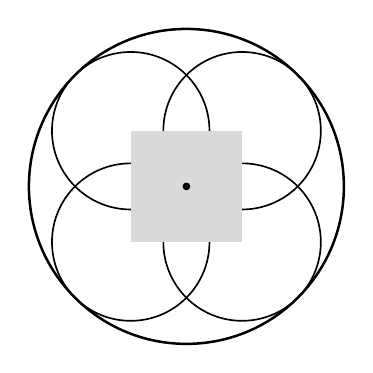
\begin{tikzpicture}[scale=2.0, semithick]
  \draw[line width=0.9pt] (0,0) circle[radius=1];
  \foreach \a in {45,135,225,315} {
    \draw (\a:0.5) circle[radius=0.5];
  }
  \fill[gray!30] (0.354,0.354) -- (0.354,-0.354) -- (-0.354,-0.354) -- (-0.354,0.354) -- cycle;
  \fill (0,0) circle (0.7pt);
\end{tikzpicture}
